\documentclass[handout]{beamer}


\usetheme{default}
\usepackage{subfigure}
\usepackage{amsmath}
\usepackage{Sweave}
\usepackage{graphicx}
\usepackage{color}
\usepackage{multicol}
\usepackage{bm}


\author{Patrick Lam}
\title{Non-Conjugate Models and Grid Approximations}
\date{}
%\date{September 29, 2008}

\begin{document}


\newcommand{\red}{\textcolor{red}}
\newcommand{\blue}{\textcolor{blue}}
\newcommand{\purple}{\textcolor{purple}}

\frame{\titlepage}

\begin{frame}
\frametitle{Outline}
\tableofcontents
\end{frame}

\section{The Binomial Model with a Non-Conjugate Prior}

\begin{frame}
\frametitle{Outline}
\tableofcontents[currentsection]
\end{frame}

\begin{frame}
\frametitle{The Binomial Example}
\pause
Suppose we have vector of data on voter turnout for a random sample of $n$
voters in the 2004 US Presidential election.   \\
\pause
\bigskip
We can model the voter turnout with a binomial model.\\
\pause
\begin{equation*}
Y \sim \mathrm{Binomial}(n, \pi)
\end{equation*}
\pause
\bigskip
Quantity of interest: $\pi$ (voter turnout)\\
\pause
\bigskip
Assumptions:
\pause
\begin{itemize}
\item Each voter's decision to vote follows the Bernoulli
distribution. \pause
\item Each voter has the same probability of voting.  \pause
(unrealistic) \pause
\item Each voter's decision to vote is independent.  \pause (unrealistic)
\end{itemize}
\end{frame}

\begin{frame}[fragile]
\frametitle{Non-Conjugate Priors}
\pause
Suppose we decide not to use the conjugate beta prior, but rather a
\textcolor{red}{non-conjugate prior}.  \pause  The \textcolor{blue}{posterior} will no longer be in a convenient distributional form.\\
\pause
\bigskip
For example, the \textcolor{red}{triangle prior} we saw in class:
\pause
\begin{eqnarray*}
\textcolor{red}{p(\pi) = \left\lbrace \begin{array}{ll} 8\pi & \mathrm{if} \;
0 \le \pi < 0.25 \\
\frac{8}{3} - \frac{8}{3} \pi & \mathrm{if} \; 0.25 \le \pi \le 1 \\
0 & \mathrm{otherwise} \end{array} \right. }
\end{eqnarray*}
\pause
\tiny{
\begin{Schunk}
\begin{Sinput}
> triangle.prior <- function(x) {
+     if (x >= 0 && x < 0.25) 
+         8 * x
+     else if (x >= 0.25 && x <= 1) 
+         8/3 - 8 * x/3
+     else 0
+ }
\end{Sinput}
\end{Schunk}
}
\pause
\normalsize
To find the \textcolor{blue}{posterior}, we need to use grid approximation methods.
\end{frame}

\begin{frame}[fragile]
\frametitle{Grid Approximation Method}
\pause
We can find the \textcolor{cyan}{unnormalized posterior} simply multiplying the
binomial likelihood and the
\textcolor{red}{non-conjugate prior}.  
\pause
\medskip
\tiny
\begin{Schunk}
\begin{Sinput}
> posterior.function <- function(theta, n, y) {
+     (theta^y) * (1 - theta)^(n - y) * triangle.prior(theta)
+ }
\end{Sinput}
\end{Schunk}
\normalsize
\bigskip
\pause To find the \textcolor{blue}{normalized
posterior}, we need to estimate the \textcolor{brown}{normalizing
constant}, which I denote as \textcolor{brown}{c}.  \\
\pause
\bigskip
\textcolor{brown}{c} is simply the area under the \textcolor{cyan}{unnormalized
posterior}. \\
\pause
\bigskip
Once we find \textcolor{brown}{c}, we can simply divide all the
ordinates (density values) of the \textcolor{cyan}{unnormalized posterior} by
\textcolor{brown}{c} to get the ordinates of the \textcolor{blue}{normalized
posterior}. \\
\pause
\bigskip
There are two ways to get the \textcolor{blue}{normalized posterior} in R.
\end{frame}


\begin{frame}[fragile]
\frametitle{Univariate Grid Approximation Method (harder way)}
\pause
\begin{itemize}
\item[1.] Divide the area under the \textcolor{cyan}{unnormalized posterior} into $m$ grids,
each of width $k$, starting from $\pi_0$, which is a value of $\pi$
that is at the far left of the parameter space.
\pause
\medskip
\tiny
\begin{Schunk}
\begin{Sinput}
> m <- 100
> grid.points <- seq(from = 0, to = 1, length.out = m)
\end{Sinput}
\end{Schunk}
\bigskip
\normalsize
\pause
\item[2.] Evaluate each grid point $(\pi_0 + k), (\pi_0 + 2k), \dots, (\pi_0 + mk)$ at the \textcolor{cyan}{unnormalized posterior}: $p(y|\pi_0 +
ik) \textcolor{red}{p(\pi_0 + ik)}$.
\pause
\medskip
\tiny
\begin{Schunk}
\begin{Sinput}
> unnormal.post.ord <- posterior.function(theta = grid.points, 
+     n = 500, y = 285)
\end{Sinput}
\end{Schunk}
\normalsize
\end{itemize}
\end{frame}

\begin{frame}[fragile]
\begin{itemize}
\item[3.] Estimate \textcolor{brown}{c} (area under the \textcolor{cyan}{unnormalized posterior}) as the sum of the areas of
rectangles of width $k$ and height at the \textcolor{cyan}{unnormalized posterior} ordinates:
\pause
\begin{eqnarray*}
\textcolor{brown}{c} \approx \sum_{i=1}^m k \; \textcolor{cyan}{p(y|\pi_0 + ik) p(\pi_0 + ik)}
\end{eqnarray*} 
\pause
\tiny
\begin{Schunk}
\begin{Sinput}
> k <- 1/m
> normal.constant <- sum(k * unnormal.post.ord)
\end{Sinput}
\end{Schunk}
\pause
\bigskip
\normalsize
\item[4.] Divide the \textcolor{cyan}{unnormalized posterior} ordinates by
\textcolor{brown}{c} to get \textcolor{blue}{normalized posterior} ordinates. 
\pause
\medskip
\tiny
\begin{Schunk}
\begin{Sinput}
> post.ord <- unnormal.post.ord/normal.constant
\end{Sinput}
\end{Schunk}
\end{itemize}
\normalsize
\end{frame}

\begin{frame}[fragile]
We can use the \textcolor{blue}{normalized posterior} ordinates to
plot our \textcolor{blue}{normalized posterior}.
\pause
\medskip
\tiny
\begin{Schunk}
\begin{Sinput}
> plot(x = grid.points, y = post.ord, type = "l", col = "blue", 
+     xlab = expression(pi), ylab = expression(paste("p(", pi, 
+         "|y)")), main = "Normalized Posterior with Triangle Prior")
\end{Sinput}
\end{Schunk}
\begin{figure}[!htp]
\begin{center}
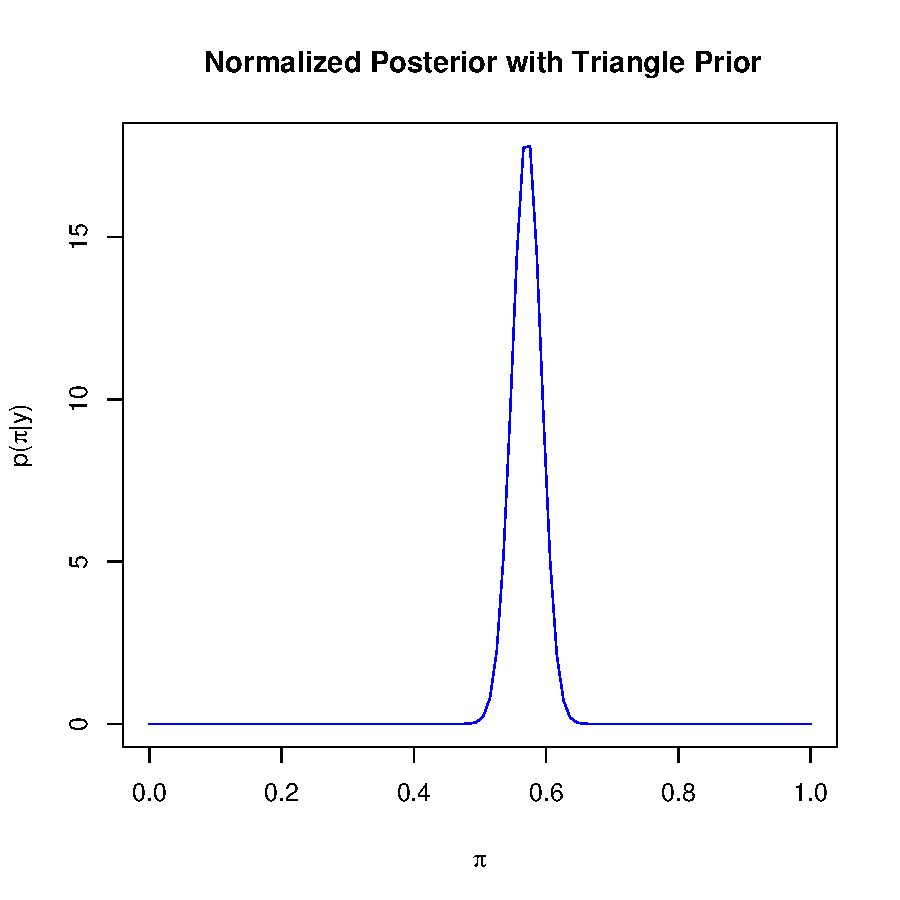
\includegraphics[width = 2in, height = 2in]{grid-trianglepost.pdf}
\end{center}
\end{figure}
\normalsize
\end{frame}

\begin{frame}[fragile]
We can also sample from our \textcolor{blue}{normalized posterior}. 
\tiny
\medskip 
\pause
\begin{Schunk}
\begin{Sinput}
> set.seed(12345)
> posterior.triangle.1 <- sample(grid.points, size = 10000, replace = T, 
+     prob = post.ord)
\end{Sinput}
\end{Schunk}
\normalsize
\pause
\bigskip
Note that the \textcolor{blue}{normalized posterior} ordinates are not
probabilities, but rather the heights of the density.  \pause However, the
{\tt sample()} function in R will normalize the ordinates into probabilities.
\end{frame}

\begin{frame}[fragile]
\frametitle{Univariate Grid Approximation Method (easier way)}
\pause

Since the {\tt sample()} function in R will automatically normalize
unnormalized probability values, we do not need steps 3 and 4.
\bigskip
\pause
\begin{itemize}
\item[1.] Divide the \textcolor{cyan}{unnormalized posterior} area into $m$ grids.
\pause
\medskip
\tiny
\begin{Schunk}
\begin{Sinput}
> m <- 100
> grid.points <- seq(from = 0, to = 1, length.out = m)
\end{Sinput}
\end{Schunk}
\bigskip
\normalsize
\pause
\item[2.] Evaluate each grid point at the \textcolor{cyan}{unnormalized posterior}.
\pause
\medskip
\tiny
\begin{Schunk}
\begin{Sinput}
> unnormal.post.ord <- posterior.function(theta = grid.points, 
+     n = 500, y = 285)
\end{Sinput}
\end{Schunk}
\bigskip
\pause
\normalsize
\item[3.] Sample grid points with \textcolor{cyan}{unnormalized posterior} ordinates as
the probabilities (letting R normalize them for us).
\medskip
\pause
\tiny
\begin{Schunk}
\begin{Sinput}
> set.seed(12345)
> posterior.triangle.2 <- sample(grid.points, size = 10000, replace = T, 
+     prob = unnormal.post.ord)
> all.equal(posterior.triangle.1, posterior.triangle.2)
\end{Sinput}
\begin{Soutput}
[1] TRUE
\end{Soutput}
\end{Schunk}
\end{itemize}
\end{frame}


\section{Bayesian Regression with Grid Approximations}

\begin{frame}
\frametitle{Outline}
\tableofcontents[currentsection]
\end{frame}

\begin{frame}
\frametitle{Poisson Regression}
\pause
Suppose we had some data $\mathbf{y}$ that was the number of events in
a given period of time.  \pause We also have a covariate
$\mathbf{x}$. \pause We can do a Bayesian Poisson regression to find
the posterior for an intercept $\alpha$ and a slope $\beta$. \\
\bigskip
\pause
Let's use a couple of Normal priors on $\alpha$ and $\beta$. 
\footnotesize
\begin{eqnarray*}
\blue{\mathrm{Posterior}(\alpha, \beta)} &\propto& \prod_{i=1}^n
\mathrm{Poisson}(\lambda_i) \times \red{\mathrm{Normal}(\mu_{\alpha},
\sigma^2_{\alpha}) \times \mathrm{Normal}(\mu_{\beta}, \sigma^2_{\beta})} \\
\pause
\blue{p(\alpha, \beta | \mathbf{y}, \mathbf{x})} &\propto&
\prod_{i=1}^n \frac{e^{-\lambda_i} \lambda_i^{y_i}}{y_i !} \times
\red{\frac{1}{\sqrt{2\pi \sigma^2_{\alpha}}} \exp \left(-
\frac{(\alpha - \mu_{\alpha})^2}{2 \sigma_{\alpha}^2}\right)}\\
&\phantom{\propto}& \red{\times \frac{1}{\sqrt{2\pi \sigma^2_{\beta}}} \exp \left(-\frac{(\beta - \mu_{\beta})^2}{2 \sigma_{\beta}^2}\right)} 
\end{eqnarray*}
\end{frame}

\begin{frame}
Our covariate $x_i$ affects the mean of the Poisson likelihood
$\lambda_i$.  \\
\bigskip
\pause
Our linear predictor $\alpha + \beta x_i$ can predict negative values,
but our Poisson mean $\lambda_i$ is always positive, so we can use the
\textbf{link function} to reparameterize $\lambda_i$ so that it can take on
negative values.\\

\bigskip
\pause
For the Poisson, the link function is the natural log function:
\begin{eqnarray*}
\mathrm{ln} (\lambda_i) = \alpha + \beta x_i
\end{eqnarray*}
\pause
However, typically we use the \textbf{inverse link function} to
reparameterize $\alpha + \beta x_i$ so that it can only take on
positive values.
\pause
\begin{eqnarray*}
\lambda_i = \exp (\alpha + \beta x_i)
\end{eqnarray*}
\end{frame}

\begin{frame}
\frametitle{Common Link (and Inverse Link) Functions}
\pause
Poisson:
\begin{itemize}
\item Link: $\mathrm{ln} (\lambda_i) = \alpha + \beta x_i$
\item Inverse Link: $\lambda_i = \exp (\alpha + \beta x_i)$
\end{itemize}
\pause
Logit:
\begin{itemize}
\item Link: $\mathrm{ln} \left( \frac{\pi_i}{1-\pi_i} \right) = \alpha +
\beta x_i$
\item Inverse Link: $\pi_i = \frac{e^{\alpha + \beta x_i}}{1 + e^{\alpha + \beta x_i}} = \frac{1}{1 + e^{-(\alpha + \beta x_i)}}$
\end{itemize}
\pause
Probit:
\begin{itemize}
\item Link: $\Phi^{-1}(\pi_i) = \alpha + \beta x_i$
\item Inverse Link: $\pi_i = \Phi(\alpha + \beta x_i)$
\end{itemize}
\end{frame}

\begin{frame}
\frametitle{Back to our Poisson Model}
\pause
So our posterior is 
\footnotesize
\begin{eqnarray*}
\blue{p(\alpha, \beta | \mathbf{y}, \mathbf{x})} &\propto&
\prod_{i=1}^n \frac{e^{-\lambda_i} \lambda_i^{y_i}}{y_i !} \times
\red{\frac{1}{\sqrt{2\pi \sigma^2_{\alpha}}} \exp \left(-
\frac{(\alpha - \mu_{\alpha})^2}{2 \sigma_{\alpha}^2}\right)}\\
&\phantom{\propto}& \red{\times \frac{1}{\sqrt{2\pi \sigma^2_{\beta}}} \exp \left(-\frac{(\beta - \mu_{\beta})^2}{2 \sigma_{\beta}^2}\right)} 
\end{eqnarray*}
\pause
\normalsize
Using our inverse link function, we get
\footnotesize
\begin{eqnarray*}
\blue{p(\alpha, \beta | \mathbf{y}, \mathbf{x})} &\propto&
\prod_{i=1}^n \frac{e^{-\exp (\alpha + \beta x_i)} (\exp (\alpha +
\beta x_i))^{y_i}}{y_i !} \times
\red{\frac{1}{\sqrt{2\pi \sigma^2_{\alpha}}} \exp \left(-
\frac{(\alpha - \mu_{\alpha})^2}{2 \sigma_{\alpha}^2}\right)}\\
&\phantom{\propto}& \red{\times \frac{1}{\sqrt{2\pi \sigma^2_{\beta}}} \exp \left(-\frac{(\beta - \mu_{\beta})^2}{2 \sigma_{\beta}^2}\right)} 
\end{eqnarray*}
\end{frame}

\begin{frame}[fragile]
Computationally, we like to work with the log posterior (we can add
small numbers rather than multiplying) and then exponentiate.\\
\bigskip
\pause 
Our log posterior is
\footnotesize
\begin{eqnarray*}
\blue{\mathrm{ln} \; p(\alpha, \beta | \mathbf{y}, \mathbf{x})} &\propto&
\sum_{i=1}^n \mathrm{ln} \left( \frac{e^{-\exp (\alpha + \beta x_i)}
(\exp (\alpha + \beta x_i))^{y_i}}{y_i !} \right) \\
&\phantom{\propto}& \red{ + \mathrm{ln}
\left( \frac{1}{\sqrt{2\pi \sigma^2_{\alpha}}} \exp  \left(-\frac{(\alpha -
\mu_{\alpha})^2}{2 \sigma_{\alpha}^2}\right) \right) }\\ 
&\phantom{\propto}&  \red{+ \mathrm{ln} \left( \frac{1}{\sqrt{2\pi
\sigma^2_{\beta}}} \exp \left(-\frac{(\beta - \mu_{\beta})^2}{2
\sigma_{\beta}^2}\right) \right)} 
\end{eqnarray*}
\normalsize
\pause
We can combine and simplify a bunch of terms $\dots$ \pause or we can
use some canned R functions.
\end{frame}

\begin{frame}[fragile]
\footnotesize
\begin{eqnarray*}
\blue{\mathrm{ln \; Posterior}(\alpha, \beta)} &\propto& \sum_{i=1}^n
\mathrm{ln \; Poisson}(\exp (\alpha + \beta x_i)) + \red{\mathrm{ln \;
Normal}(\mu_{\alpha}, \sigma^2_{\alpha}) } \\
&\phantom{\propto}& \red{+ \; \mathrm{ln \; Normal}(\mu_{\beta}, \sigma^2_{\beta})} \\
\end{eqnarray*}
\pause
\tiny
\begin{Schunk}
\begin{Sinput}
> poisson.posterior <- function(theta, y, x, prior.mean.a, prior.var.a, 
+     prior.mean.b, prior.var.b) {
+     a <- theta[1]
+     b <- theta[2]
+     lambda <- exp(a + b * x)
+     log.like <- sum(dpois(y, lambda = lambda, log = T))
+     log.prior.a <- dnorm(a, mean = prior.mean.a, sd = sqrt(prior.var.a), 
+         log = T)
+     log.prior.b <- dnorm(b, mean = prior.mean.b, sd = sqrt(prior.var.b), 
+         log = T)
+     log.post <- log.like + log.prior.a + log.prior.b
+     return(exp(log.post))
+ }
\end{Sinput}
\end{Schunk}
\normalsize 
\end{frame}

\begin{frame}[fragile]
\frametitle{An Example}
\pause
Let's do an example using the {\tt sanction} dataset from the {\tt
Zelig} library.
\pause
\tiny
\begin{Schunk}
\begin{Sinput}
> library(Zelig)
> data(sanction)
\end{Sinput}
\end{Schunk}
\bigskip
\pause
\normalsize
Our dependent variable is the number of sanctions, and our covariate
is level of cooperation.
\pause
\tiny
\begin{Schunk}
\begin{Sinput}
> y.vec <- sanction$num
> x.vec <- sanction$coop
\end{Sinput}
\end{Schunk}
\normalsize
\bigskip
\pause
For the priors on $\alpha$ and $\beta$, let's use two Normal(0,20)
distributions, which are relatively flat.
\tiny
\pause
\begin{Schunk}
\begin{Sinput}
> mu.a <- mu.b <- 0
> sigma2.a <- sigma2.b <- 20
\end{Sinput}
\end{Schunk}
\end{frame}

\begin{frame}[fragile]
Since we don't know the normalizing constant and we don't have
conjugacy, we need to simulate from the posterior somehow.  \\
\pause
\bigskip
Fortunately, since our posterior is bivariate, we can still use the
grid approximation method fairly easily. \\
\pause
\bigskip
One possible problem with a grid approximation approach is that our
parameter space is unbounded.  \pause If our grid misses an area of the
posterior that has high density, then our simulations will be incorrect.\\ 
\pause
\bigskip
One reasonable solution is to center our grid at the MLE.
\pause
\bigskip
\pause
\tiny
\begin{Schunk}
\begin{Sinput}
> mle <- glm(num ~ coop, data = sanction, family = poisson)$coef
> mle.se <- summary(glm(num ~ coop, data = sanction, 
+     family = poisson))$coef[, 2]
\end{Sinput}
\end{Schunk}
\end{frame}

\begin{frame}[fragile]
I then create a grid that is centered at the MLE and spans an
arbitrary 5 standard errors away on both sides.
\pause
\medskip
\tiny
\begin{Schunk}
\begin{Sinput}
> grid.a <- seq(from = mle[1] - 5 * mle.se[1], to = mle[1] + 5 * 
+     mle.se[1], length.out = 200)
> grid.b <- seq(from = mle[2] - 5 * mle.se[2], to = mle[2] + 5 * 
+     mle.se[2], length.out = 200)
> grid.points <- expand.grid(grid.a, grid.b)
\end{Sinput}
\end{Schunk}
\pause
\normalsize
\bigskip
Once we have the grid points, we can evaluate at the unnormalized posterior
\tiny
\pause
\medskip
\begin{Schunk}
\begin{Sinput}
> post.ord <- apply(grid.points, MARGIN = 1, FUN = poisson.posterior, 
+     y = y.vec, x = x.vec, prior.mean.a = mu.a, prior.var.a = sigma2.a, 
+     prior.mean.b = mu.b, prior.var.b = sigma2.b)
\end{Sinput}
\end{Schunk}
\pause
\bigskip
\normalsize
and then sample (letting R normalize for us) to get the simulated posterior.
\pause
\medskip
\tiny
\begin{Schunk}
\begin{Sinput}
> sample.indices <- sample(1:nrow(grid.points), size = 10000, replace = T, 
+     prob = post.ord)
> sim.posterior <- grid.points[sample.indices, ]
\end{Sinput}
\end{Schunk}
\normalsize
\end{frame}

\begin{frame}[fragile]
\frametitle{Posterior Summary}
\pause
Our posterior means are comparable to our MLEs.
\medskip
\pause
\tiny
\begin{Schunk}
\begin{Sinput}
> posterior.means <- colMeans(sim.posterior)
> posterior.means
\end{Sinput}
\begin{Soutput}
  Var1   Var2 
-1.007  1.207 
\end{Soutput}
\begin{Sinput}
> mle
\end{Sinput}
\begin{Soutput}
(Intercept)        coop 
     -1.003       1.207 
\end{Soutput}
\end{Schunk}
\normalsize
\bigskip
\pause
as well as our posterior standard deviations and our MLE SEs.
\medskip
\pause
\tiny
\begin{Schunk}
\begin{Sinput}
> posterior.sd <- apply(sim.posterior, MARGIN = 2, FUN = sd)
> posterior.sd
\end{Sinput}
\begin{Soutput}
  Var1   Var2 
0.1466 0.0453 
\end{Soutput}
\begin{Sinput}
> mle.se
\end{Sinput}
\begin{Soutput}
(Intercept)        coop 
    0.14602     0.04504 
\end{Soutput}
\end{Schunk}
\end{frame}




\end{document}
